\chapter{Procedimiento}
A continuación se describen los procesos del algoritmo que permiten solucionar el problema especificado. El código fuente está disponible de manera digital en la plataforma de GitHub \cite{LindermanDgz}.

\section{Lectura del dataset}
Se comienza leyendo el dataset que contiene información que ha sido etiquetada de manera manual por los autores del mismo. Este proceso se describe en \Cref{code:load_dataset}.

\begin{listing}[!ht]
\inputminted{python}{code_listings/load_dataset.py}
\caption{Cargar las anotaciones del dataset}
\label{code:load_dataset}
\end{listing}

Utilizando la biblioteca \texttt{json} de Python leémos el archivo \texttt{RoCoLE.json} (originalmente \texttt{Annotations/RoCoLE-json.json}). La variable \texttt{annotations} contiene la información necesaria para contruir nuestro conjunto de datos de prueba (véase \Cref{table:required_annotations}).

\begin{table}[h!]
\centering
\begin{tabular}{|l|l|}
\hline 
\textbf{Anotación} & \textbf{Descripción} \\ 
\hline 
ID & Identificador de la hoja \\ 
\hline 
Label.Leaf.0.state & Estado de la hoja como saludable o infectada \\ 
\hline 
Label.classification & Clasificación de la hoja o nivel de afectación \\ 
\hline 
Label.Leaf.0.geometry & Puntos (x,y) que determinan el contorno de la hoja \\ 
\hline 
\end{tabular}
\caption{Anotaciones del dataset}
\label{table:required_annotations}
\end{table}

\subsection{La clase CoffeeLeaf}
A continuación creamos una clase llamada \texttt{CoffeeLeaf} la cual se encarga de contener los datos proporcionados en las anotaciones y que representa a una hoja de café. Los atributos de esta clase pueden observarse en \Cref{code:coffee_leaf}.

\begin{listing}[!ht]
\inputminted{python}{code_listings/coffee_leaf.py}
\caption{La clase CoffeeLeaf}
\label{code:coffee_leaf}
\end{listing}

Una vez creada la clase \texttt{CoffeeLeaf} y leído los datos del dataset, procedemos a crear la lista \texttt{coffee\_leaves} utilizando los datos de la \Cref{table:required_annotations}, tal como se muestra en \Cref{code:coffee_leaves}. El directorio \texttt{../rocole\_photos/} contiene los archivos \texttt{.jepg} del dataset (\texttt{Annotations/RoCoLe-voc.tar.gz/export}).

\begin{listing}[!ht]
\inputminted{python}{code_listings/coffee_leaves.py}
\caption{Lista de objetos CoffeLeaf}
\label{code:coffee_leaves}
\end{listing}

\section{Procesado de la imagen}
Una vez creada la lista \texttt{coffee\_leaves} iniciamos el procesamiento de las imagénes a través de la función \texttt{process} (\Cref{code:process}) de la clase \texttt{CoffeeLeaf}. Véase \Cref{code:process_iteration}.

\begin{listing}[!ht]
\inputminted{python}{code_listings/process.py}
\caption{Función process del la clase CoffeeLeaf}
\label{code:process}
\end{listing}

\begin{listing}[!ht]
\inputminted{python}{code_listings/process_iteration.py}
\caption{Iniciar procesamiento de las imágenes}
\label{code:process_iteration}
\end{listing}

\subsection{Conversión de BGR a RGB}
Debido a que cuando creamos los objetos \texttt{CoffeeLeaf} el argumento \texttt{image\_bgr} pasa datos de una imagen en color \textsf{BGR} (Blue, Green, Red), que es la representación de color por defecto de \textit{OpenCV}, y ya que \textit{matplotlib}, la herramienta para la visualización de las imágenes, utiliza una representación \textsf{RGB} (Red, Green, Blue), una conversión de color es necesaria. Véase \Cref{code:bgr_to_rgb}.

\begin{listing}[!ht]
\inputminted{python}{code_listings/bgr_to_rgb.py}
\caption{Convertir imgen BGR a RGB}
\label{code:bgr_to_rgb}
\end{listing}

El resultado de esta conversión permite visualizar la imagen original (\Cref{img:original}).

\begin{figure}[hbtp]
\centering
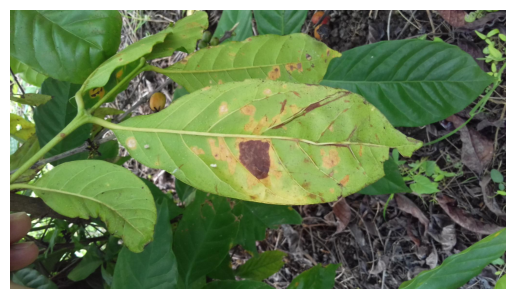
\includegraphics[scale=1]{images/original_image.png}
\caption{Imagen original en RGB}
\label{img:original}
\end{figure}

\subsection{Creación de las regiones de interés}

\subsection{Creación de la máscara}
\begin{listing}[!ht]
\inputminted{python}{code_listings/mask.py}
\caption{Crear máscara}
\label{code:mask}
\end{listing}

\subsection{Enmascaramiento de las regiones de interés}
\begin{listing}[!ht]
\inputminted{python}{code_listings/masked_roi.py}
\caption{Enmascarar las regiones de interés}
\label{code:masked_roi}
\end{listing}

\subsection{Histograma de las regiones de interés}
\begin{listing}[!ht]
\inputminted{python}{code_listings/histogram.py}
\caption{Cálcular histograma de la región de interés}
\label{code:histogram}
\end{listing}

\subsection{Segmentación de la imagen}
\begin{listing}[!ht]
\inputminted{python}{code_listings/segmentation.py}
\caption{Segmentar la región de interés}
\label{code:segmentation}
\end{listing}

\subsection{Clasificación de la hoja}
\begin{listing}[!ht]
\inputminted{python}{code_listings/categorize.py}
\caption{Clasificar hoja de café}
\label{code:categorize}
\end{listing}

\section{Presentación de los datos}

\subsection{Resumen}
\begin{listing}[!ht]
\inputminted{python}{code_listings/show_summary.py}
\caption{Mostrar resumen de la clasificación}
\label{code:show_summary}
\end{listing}

\subsection{Imagen original}
\begin{listing}[!ht]
\inputminted{python}{code_listings/show_original_image.py}
\caption{Mostrar imagen original}
\label{code:show_original_image}
\end{listing}

\subsection{Máscara}
\begin{listing}[!ht]
\inputminted{python}{code_listings/show_mask.py}
\caption{Mostrar máscara}
\label{code:show_mask}
\end{listing}

\subsection{Regiones de interés}
\begin{listing}[!ht]
\inputminted{python}{code_listings/show_roi.py}
\caption{Mostrar regiones de interés}
\label{code:show_roi}
\end{listing}

\subsection{Imagen segmentada}
\begin{listing}[!ht]
\inputminted{python}{code_listings/show_segmentation.py}
\caption{Mostrar segmentación de la imagen}
\label{code:show_segmentation}
\end{listing}

\subsection{Histograma}
\begin{listing}[!ht]
\inputminted{python}{code_listings/show_histogram.py}
\caption{Mostrar histograma de la región de interés}
\label{code:show_histogram}
\end{listing}